\documentclass[tikz,border=4pt]{standalone}
\usepackage{amsmath,amssymb}
\usetikzlibrary{arrows.meta,positioning,fit,backgrounds}
\begin{document}
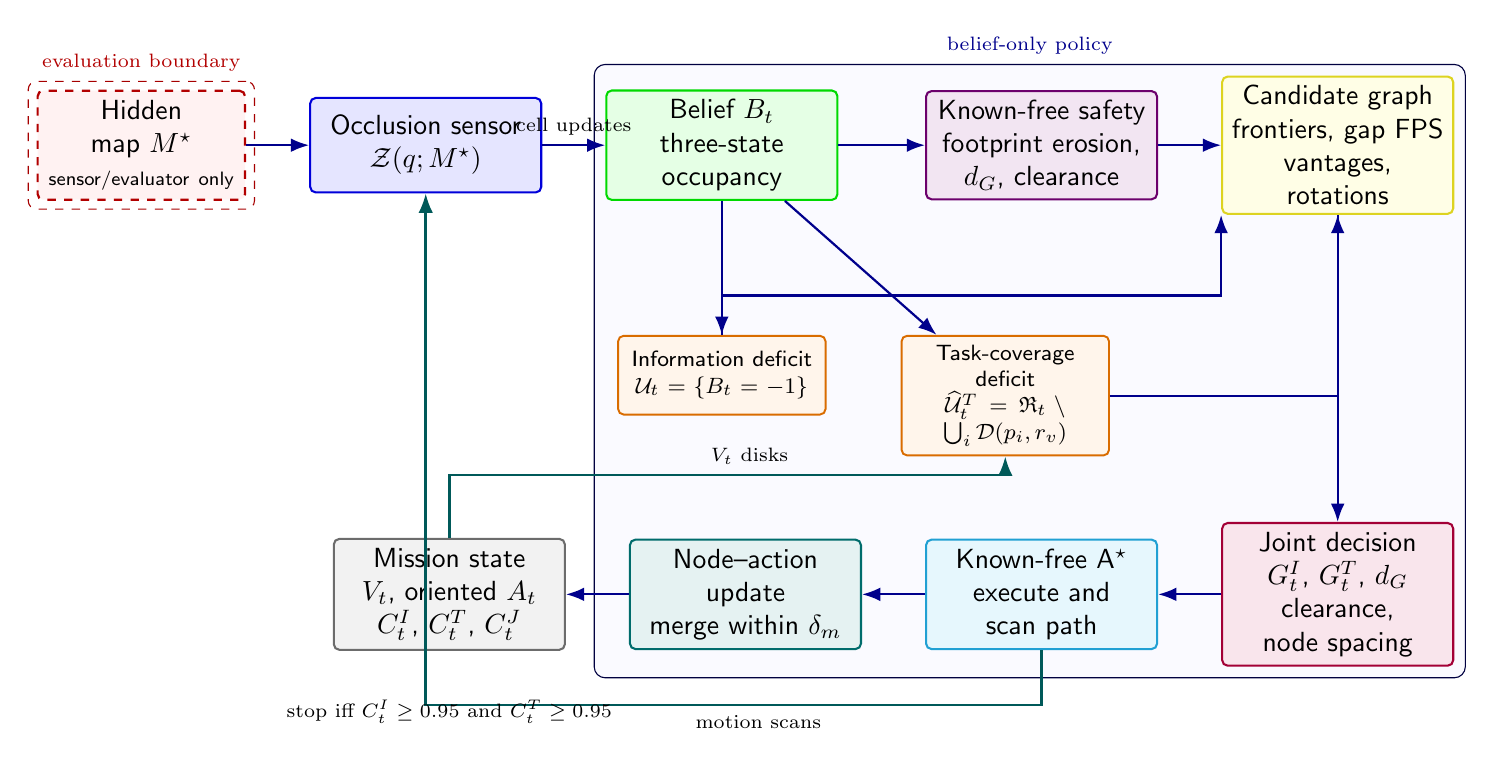
\begin{tikzpicture}[
  font=\sffamily,
  >=Latex,
  node distance=7mm and 8mm,
  block/.style={draw=#1!85!black, fill=#1!10, rounded corners=2pt,
    line width=.75pt, align=center, minimum height=12mm, text width=27mm},
  small/.style={draw=#1!85!black, fill=#1!8, rounded corners=2pt,
    line width=.7pt, align=center, minimum height=10mm, text width=24mm,
    font=\sffamily\footnotesize},
  flow/.style={-Latex, line width=.8pt, draw=blue!55!black},
  loop/.style={-Latex, line width=.9pt, draw=teal!70!black},
  eval/.style={draw=red!70!black, fill=red!5, dashed, rounded corners=2pt,
    line width=.8pt, align=center, minimum height=12mm, text width=24mm}
]

\node[eval] (truth) {Hidden map $M^\star$\\\scriptsize sensor/evaluator only};
\node[block=blue, right=of truth] (sensor) {Occlusion sensor\\$\mathcal Z(q;M^\star)$};
\node[block=green, right=of sensor] (belief) {Belief $B_t$\\three-state occupancy};

\node[small=orange, below=17mm of belief] (igap)
  {Information deficit\\$\mathcal U_t=\{B_t=-1\}$};
\node[small=orange, below=17mm of belief, xshift=36mm] (tgap)
  {Task-coverage deficit\\$\widehat{\mathcal U}_t^T=\mathfrak R_t\setminus\!\bigcup_i\mathcal D(p_i,r_v)$};

\node[block=violet, right=11mm of belief] (reach)
  {Known-free safety\\footprint erosion, $d_G$, clearance};
\node[block=yellow, right=of reach] (cand)
  {Candidate graph\\frontiers, gap FPS\\vantages, rotations};

\node[block=purple, below=39mm of cand] (score)
  {Joint decision\\$G_t^I$, $G_t^T$, $d_G$\\clearance, node spacing};
\node[block=cyan, left=of score] (astar)
  {Known-free A$^\star$\\execute and scan path};
\node[block=teal, left=of astar] (assoc)
  {Node--action update\\merge within $\delta_m$};
\node[block=gray, left=of assoc] (state)
  {Mission state\\$V_t$, oriented $A_t$\\$C_t^I$, $C_t^T$, $C_t^J$};

\draw[flow] (truth) -- (sensor);
\draw[flow] (sensor) -- node[above, font=\scriptsize]{cell updates} (belief);
\draw[flow] (belief) -- (reach);
\draw[flow] (reach) -- (cand);
\draw[flow] (belief) -- (igap);
\draw[flow] (belief) -- (tgap);
\draw[flow] (igap.north) -- ++(0,5mm) -| (cand.south west);
\draw[flow] (tgap.east) -| (cand.south);
\draw[flow] (cand) -- (score);
\draw[flow] (score) -- (astar);
\draw[flow] (astar) -- (assoc);
\draw[flow] (assoc) -- (state);
\draw[loop] (astar.south) -- ++(0,-7mm) -| node[pos=.23, below, font=\scriptsize]{motion scans} (sensor.south);
\draw[loop] (state.north) -- ++(0,8mm) -| node[pos=.27, above, font=\scriptsize]{$V_t$ disks} (tgap.south);
\node[below=5mm of state, font=\scriptsize, align=center]
  {stop iff $C_t^I\ge0.95$ and $C_t^T\ge0.95$};

\begin{scope}[on background layer]
  \node[draw=red!65!black, dashed, rounded corners=3pt, fit=(truth),
    inner sep=3pt, label={[font=\scriptsize,text=red!70!black]above:evaluation boundary}] {};
  \node[draw=blue!25!black, rounded corners=4pt, fit=(belief)(reach)(cand)(igap)(tgap)(score),
    inner sep=4pt, fill=blue!2,
    label={[font=\scriptsize,text=blue!55!black]above:belief-only policy}] {};
\end{scope}

\end{tikzpicture}
\end{document}
